\documentclass{article-hermes}	

\usepackage[utf8x]{inputenc}
\usepackage[T1]{fontenc}
\usepackage{pgf, tikz}
\usepackage{multirow}
\usetikzlibrary{arrows,shapes,positioning}

\title[$  $]{Recherche de conversations dans les réseaux sociaux : 
modélisation et expérimentations sur Twitter.}

\author{
%Nawal  Ould Amer\fup{*,**} \andauthor Philippe Mulhem \fup{*} \andauthor Mathias Géry \fup{**}  
} 

\address{%
%\fup{*}{LIG - Université de Grenoble : Nawal.Ould-Amer, Philippe.Mulhem@imag.fr} \\
%\fup{**}{Laboratoire Hubert-Curien - Université de Saint-Étienne : Mathias.Gery@univ-st-etienne.fr}
}

\resume{
La problématique étudiée dans cet article est celle de l'indexation et de la recherche de conversations dans les réseaux sociaux. Une conversation est un ensemble de messages échangés entre utilisateurs, à la suite d'un message initial. La démarche proposée se base sur une modélisation probabiliste, et détaille en particulier l'utilisation d'informations sociales dans le réseau Twitter. Notre proposition est évaluée sur un corpus de conversations contenant plus de 50 000 tweets, et sur un ensemble de 15 requêtes tirées pour partie des campagnes TREC Microblog \cite{trec2013}. Les résultats obtenus en combinant les éléments de contenu et les éléments sociaux sur ce corpus sont statistiquement significativement meilleurs que ceux de notre approche utilisant le contenu seul ainsi que ceux d'une approche à base de BM25.
}

\abstract{
The problem considered in this paper tackles the indexing and retrieval of conversations in social networks. A conversation is a set of messages exchanged between users, following an initial message. The proposed approach is based on a probabilistic modeling, focusing specifically on the use of social information available on the Twitter platform. Our proposal is evaluated on a corpus of conversations with more than 50,000 tweets, and a set of 15 queries drawn partly from TREC Microblog campaigns \cite{trec2013}. The results obtained on this corpus are statistically significantly better than two content-only probabilistic approaches.
}

\motscles{
Indexation de conversation,
Recherche de conversation,
Modèle probabiliste,
Collection de test,
Réseau social.
}

\keywords{
Conversation indexing,
Conversation retrieval,
Probabilistic modeling,
Test collection,
Social Network.
}

%\date{}
\begin{document}
  
\maketitlepage

%%%%%%%% FAKE TEXT %%%%%%%%%%%%%%%
\newcommand{\fakesentence}{Attention à ce que les figures et les tableaux ne débordent pas dans les marges. }
\newcommand{\fakeparagraph}{
\fakesentence
\fakesentence
\fakesentence
\fakesentence
\fakesentence
\fakesentence
}
%%%%%%%%%%%%%%%%%%%%%%%%%%%%%%

\section{Introduction}

La recherche d'information sociale a pour objectif de retrouver des documents qui correspondent à un besoin d'information d'un utilisateur, tout en intégrant des éléments provenant de la participation des utilisateurs à des réseaux sociaux. Plutôt que de se limiter à la recherche de documents atomiques (comme des tweets dans Twitter par exemple), nous considérons ici qu'un élément informatif plus pertinent pour la recherche d'information sociale est la recherche de {\it conversations} sociales, une conversation étant un ensemble de posts échangés par des utilisateurs sur un sujet donné. 

\label{sec:convtw}
Une conversation $c$ dans le microblog Twitter est un ensemble de tweets échangés entre les blogueurs $b_j$ (cf. figure~\ref{fig:conversation}). Chaque tweet est publié à un instant donné en réponse aux tweets plus anciens (sauf pour le tweet initial). Par exemple, le tweet $t_4$ est une réponse au tweet $t_0$. Les blogueurs sont liés par des relations d'abonnements. Un blogueur a la possibilité de publier un \textit{tweet} à ses abonnées (\textit{followers}), de rediffuser un \textit{tweet} d'un autre blogueur (\textit{``RT''}), en ajoutant éventuellement un commentaire, de répondre à un \textit{tweet} (\textit{``@username''}), de mentionner un blogueur dans un tweet (\textit{@mention}), de mettre un \textit{tweet} en favoris (\textit{star}), d'ajouter dans le \textit{tweet} des mots-clés appelés \textit{hashtags} (\textit{\#motclé}) et de partager une ressource Web (\textit{url}). Une conversation $c_1$ contient donc un ensemble de tweets $t_0, t_1, ..., t_5$ qui sont publiés par les blogueurs $b_1,b_2,...,b_4$. Le blogueur $b_1$ a publié le tweet $t_0$ qui est le tweet initial de la conversation $c_1$. Le blogueur $b_2$ répond \textit{``Reply''} au tweet $t_3$ en publiant le tweet $t_5$ qui comporte le hashtag ($\#1$) et l'url ($url_1$). Les blogueurs $b_2$ et $b_4$ ont retweeté le tweet $t_4$ publié par le blogueur $b_3$ et le blogueur $b_3$ a mis en favoris le tweet $t_3$.




\begin{figure}[h]
\caption{\label{fig:conversation}Exemple de conversation dans le microblog Twitter}
\smallskip
\begin{center}
%\caption{\label{tab:queries}}
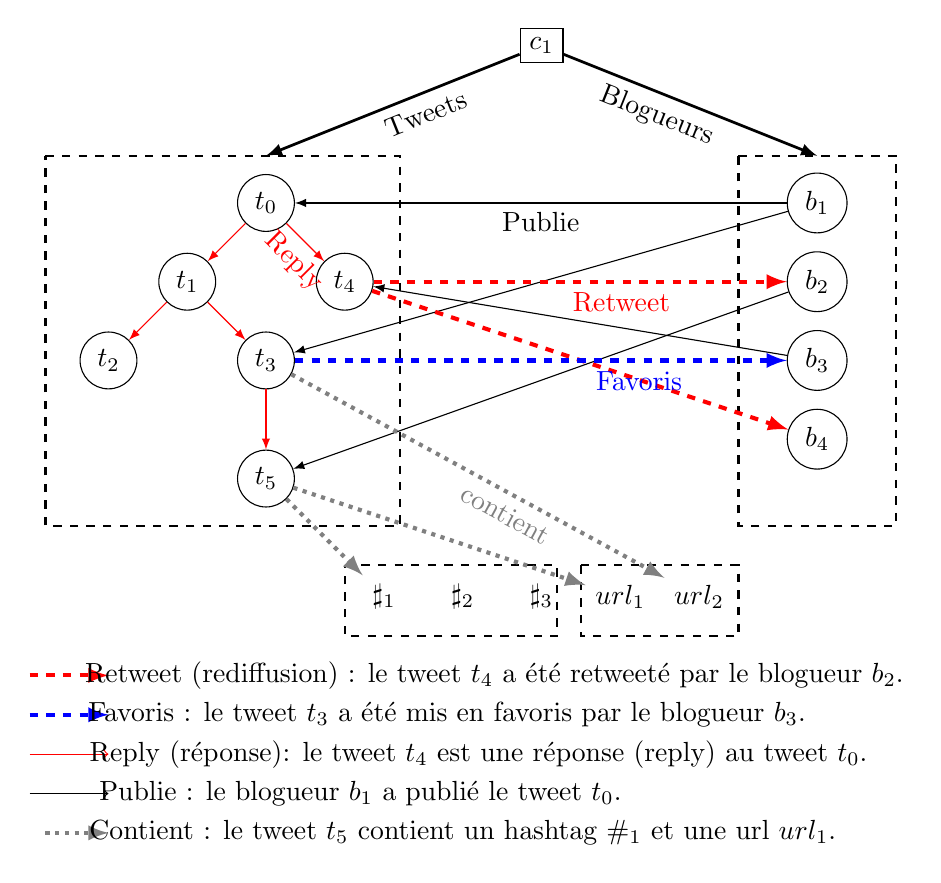
\begin{tikzpicture}
//cadre conversation 
%\draw[black, thick, dashed] (-1.5,5.1) -- (11, 5.1) --(11,-3.2) -- (-1.5, -3.2) -- (-1.5, 5.1) ; 
//conversation
\node[draw] (C) at(5.5,4.5) {$c_1$};


//hashtags et urls

// cadre urls et hashtags
\draw[black, thick, dashed] (3,-2.1) -- (5.7, -2.1) --(5.7,-3) -- (3, -3) -- (3, -2.1) ; 

\draw[black, thick, dashed] (6,-2.1) -- (8, -2.1) --(8,-3) -- (6, -3) -- (6, -2.1) ; 
// cadre tweet
\draw[black, thick, dashed] (-0.8,3.1) -- (3.7, 3.1) --(3.7,-1.6) -- (-0.8, -1.6) -- (-0.8, 3.1) ; 


// hastags et urls

\node[] (1) at(3.5,-2.5) {$\sharp_{1}$};
\node[] (2) at(4.5,-2.5) {$\sharp_{2}$};
\node[] (3) at(5.5,-2.5) {$\sharp_{3}$};
\node[] (url1) at(6.5,-2.5) {$url_{1}$};
\node[] (url2) at(7.5,-2.5) {$url_{2}$};




/// tweets
\node[draw, circle] (t0) at(2,2.5) {$t_{0}$};
\node[draw, circle] (t1) at(1,1.5) {$t_{1}$};
\node[draw, circle] (t2) at(0,0.5) {$t_{2}$};
\node[draw, circle] (t3) at(2,0.5) {$t_{3}$};
\node[draw, circle] (t4) at(3,1.5) {$t_{4}$};
\node[draw, circle] (t5) at(2,-1) {$t_{5}$};

// cadre users
\draw[black, thick, dashed] (8,3.1) -- (10, 3.1) --(10,-1.6) -- (8, -1.6) -- (8, 3.1) ; 

// users
\node[draw, circle] (u1) at(9,2.5) {$b_{1}$};
\node[draw, circle] (u2) at(9,1.5) {$b_{2}$};
\node[draw, circle] (u3) at(9,0.5) {$b_{3}$};
\node[draw, circle] (u4) at(9,-0.5) {$b_{4}$};


// publie

\draw[black,->,>=latex,](u1)--(t0)node[pos=0.5,right,below,sloped]{Publie};
\draw[black,->,>=latex,](u1)--(t3)node[pos=0.6,right,below,sloped]{};
\draw[black,->,>=latex,](u2)--(t5)node[pos=0.6,right,below,sloped]{};
\draw[black,->,>=latex,](u3)--(t4)node[pos=0.6,right,below,sloped]{};


//liens entre users et conversations

\draw[line width=1,black,->,>=latex,](C)--(9,3.1) node[pos=0.4,right,below,sloped]{Blogueurs};

//liens entres tweets et conversations
\draw[line width=1,black,->,>=latex,](C)--(2,3.1) node[pos=0.4,right,below,sloped]{Tweets};



//red reply
\draw[red,->,>=latex,](t1)--(t3)node[pos=0.6,right,below,sloped]{};
\draw[red,->,>=latex,](t0)--(t4)node[pos=0.6,right,below,sloped]{Reply};
\draw[red,->,>=latex,](t0)--(t1)node[pos=0.6,right,below,sloped]{};
\draw[red,->,>=latex,](t1)--(t2)node[pos=0.6,right,below,sloped]{};
\draw[red,->,>=latex,](t3)--(t5)node[pos=0.6,right,below,sloped]{};




// liens entre users et retweet et favoris


\draw[line width=1.5,dashed,red,->,>=latex,](t4)--(u2)node[pos=0.6,right,below,sloped]{Retweet};

\draw[line width=1.5,dashed,red,->,>=latex,](t4)--(u4)node[pos=0.6,right,below,sloped]{};

\draw[line width=1.5,dashed,blue,->,>=latex,](t3)--(u3)node[pos=0.7,right,below,sloped]{Favoris};


//liens entre tweets et hashtags et urls


\draw[line width=1.5,dotted,gray,->,>=latex,](t5)--(1)node[pos=0.6,right,below,sloped]{};


\draw[line width=1.5,dotted,gray,->,>=latex,](t5)--(url1)node[pos=0.6,right,below,sloped]{};


\draw[line width=1.5,dotted,gray,->,>=latex,](t3)--(url2)node[pos=0.6,right,below,sloped]{contient};



//légendes 
\draw[line width=1.5,dashed,red,->,>=latex,] (-1,-3.5) to (0,-3.5); \node[] (retweets) at(4.9,-3.5) {Retweet (rediffusion) : le tweet $t_4$ a été retweeté par le blogueur $b_2$.};
\draw[line width=1.5,dashed,blue,->,>=latex,] (-1,-4) to (0,-4);\node[] (favoris) at(4.3,-4) {Favoris : le tweet $t_3$ a été mis en favoris par le blogueur $b_3$.};
\draw[red,->] (-1,-4.5) to (0,-4.5);\node[] (reply) at(4.7,-4.5)  {Reply (réponse): le tweet $t_4$ est une réponse (reply) au tweet $t_0$. }; 
\draw[black,->] (-1,-5) to (0,-5);\node[] (publie) at(3.2,-5)  {Publie : le blogueur $b_1$ a publié le tweet $t_0$. };  
\draw[line width=1.5,dotted,gray,->,>=latex,] (-0.8,-5.5) to (0,-5.5);\node[] (contient) at(4.5,-5.5)  {Contient : le tweet $t_5$ contient un hashtag $\#_1$ et une url $url_1$. }; 



\end{tikzpicture}
\end{center}
\end{figure}

Une des difficultés de la recherche d'information sociale repose sur le fait qu'il existe une multitude de sources d'informations potentiellement utiles (comme le fait qu'un blogueur est populaire, qu'un tweet est considéré intéressant par de nombreux blogueurs, etc.) : la question est alors de déterminer lesquels utiliser, comment les utiliser, et comment intégrer tous ces éléments pour obtenir une recherche d'information de qualité. Le travail décrit ici vise à intégrer, dans un modèle probabiliste clair, un certain nombre d'éléments identifiés et explicités, afin de réaliser un système de recherche d'information qui fournit des bons résultats sur des corpus de conversations. 

Dans la suite de cet article, nous commençons par décrire en section~\ref{sec:eda} les travaux relatifs à notre problématique. La section~\ref{sec:modele} formalisera et présentera le modèle que nous proposons. La section \ref{sec:eval} décrira les évaluations effectuées, précédée en section~\ref{sec:colltest} par la description de la création de la collection de test sur laquelle nous avons mené nos expérimentations.
%avant de conclure.

\section{État de l'art}
\label{sec:eda}

%
\par Différents travaux se sont intéressés à la recherche de conversations dans les structures sociales comme les blogs, les forums et les microblogs (Twitter). Nous classons ces travaux en deux catégories : la première ne se basant que sur le contenu textuel des conversations et la seconde se basant sur le contenu textuel et les informations sociales. 

\par La catégorie focalisée sur l'exploitation du contenu textuel se décompose en deux approches, suivant la manière de combiner les posts d'une conversation. La fusion précoce consiste à concaténer tous les posts d'une conversation dans un seul document global et la pertinence de la conversation est donnée par le score de correspondance entre la requête  et ce document global. Dans cet axe \cite{seo2009} et \cite{elsas9} utilisent un modèle de langue sur le document global. La fusion tardive combine les scores de correspondance de chaque post de la conversation. Trois approches rentrent dans cet axe.
La première prend en compte tous les posts, applique un modèle de langue sur chaque post et fusionne les scores pour obtenir un score global pour la conversation \cite{seo2009} et \cite{elsas9}. 
La deuxième approche sélectionne les posts à utiliser avant de fusionner leur score. Cette sélection consiste à ne garder que les posts les plus pertinents lors du calcul de correspondance globale \cite{seo2009}, \cite{elsas9} et \cite{voting}.
La troisième approche consiste à utiliser la structure des conversations. Le score global est alors la combinaison d'un ou plusieurs scores provenant d'un post, d'une paire de posts ou un dialogue (ensemble de posts) \cite{seo2009}. Les résultats de ces travaux montrent que d'une part la fusion tardive donne de meilleurs résultats que la fusion précoce, et d'autre part que la prise en compte de la structure de la conversation améliore les résultats.


\par La deuxième catégorie des travaux propose de tenir compte des informations sociales offertes par les structures sociales et d'autres informations intrinsèques telles que la longueur de la conversation. \cite{Inference} proposent un modèle probabiliste qui tient compte du contenu textuel des posts, de l'autorité des auteurs, des liens entre conversations et de la taille des conversations \cite{Inference} . Ces différents facteurs sont pris en compte comme des a priori dans le modèle probabiliste. Les résultats de ces travaux montrent que l'intégration des facteurs sociaux et de la pertinence thématique améliore les résultats par rapport à la pertinence thématique seule. 

\par A notre connaissance, seuls les travaux \cite{magnani1} et \cite{magnani2} proposent de chercher des conversations dans le microblog Twitter. Ces travaux reposent sur une approche de fusion des caractéristiques suivantes : \romannumeral 1 ) la pertinence textuelle de la conversation basée sur la fusion tardive de correspondance vectorielle; \romannumeral 2) la moyenne des tailles des tweets de la conversation; \romannumeral 3) la popularité de la conversation (nombre de tweet retweetés); \romannumeral 4) la popularité des auteurs des tweets calculée par la moyenne des nombres de followers de chaque auteur; \romannumeral 6) la densité temporelle des tweets. Les auteurs montrent que l'utilisation des facteurs sociaux apporte de bons résultats mais il ne montrent pas l'apport de ces facteurs par rapport à une pertinence thématique seule. 

\par Dans cet article, nous proposons un modèle de recherche de conversations dans le microblog Twitter qui tient compte de la pertinence textuelle des tweets et de la pertinence sociale estimée au travers des informations sociales issues du réseau Twitter. Comparativement aux travaux présentés dans l'état de l'art, nous proposons un modèle probabiliste permettant d'intégrer les deux pertinences textuelle et sociale. La pertinence textuelle que nous proposons est estimée par un modèle de langue, à la différence de \cite{magnani1} et \cite{magnani2} qui utilisent un modèle vectoriel. De plus, \cite{magnani1} et \cite{magnani2} estiment l'importance des blogueurs par le nombre de leur followers, alors des travaux ont montré qu'une meilleure estimation de l'importance des blogueurs peu s'appuyer sur d'autres informations que nous choisissons d'utiliser pour évaluer la pertinence sociale (cf. présentation informelle des paramètres du modèle en Section \ref{subsec:par}).







\section{Modèle de recherche de conversations}
\label{sec:modele}


\subsection{Présentation informelle des facteurs du modèle}
\label{subsec:par}
\par Nous présentons ici les différents facteurs, autres que textuels, définis pour caractériser une conversation. Le calcul de correspondance entre une requête utilisateur et une conversation va reposer sur le contenu textuel des tweets de cette conversation, mais également sur les facteurs sociaux suivants :

\begin{itemize}
\item Participants à la conversation : nous estimons la qualité des participants au travers de leur expertise, leur influence et leur activité. L'expertise est calculée par application d'un modèle de langue inspiré de \cite{bal} et \cite{lamjedmarami}. L'influence est calculée par application du \textit{PageRank} sur les relations de retweets renforcées par les relations de favoris \cite{lamjedmarami}. L'activité d'un utilisateur dans une conversation dépend du nombre de conversations auxquelles il participe et du nombre moyen de tweets du blogueur par conversation ;

\item Contenu social : le contenu social des tweets d'une conversation tient compte des méta-données que sont les urls et les hashtags. Un tweet contenant des urls est plus informatif car il apporte une information portée par l'url (\cite{Nagmoti}, \cite{Zhao}). Un hashtag catégorise un tweet selon un contexte et augmente la visibilité du tweet \cite{Duan} ;
\item Influence sociale : elle est estimée par le nombre des tweets de la conversation qui sont mis en favoris par des blogueurs, ainsi que par le nombre de tweets de la conversation qui sont retweetés.
\end{itemize}

On remarque que la description ci-dessus utilise certaines informations spécifiques au réseau social Twitter, car ce réseau est celui auquel nous nous intéressons. On peut cependant noter que pour d'autres réseaux sociaux, des informations équivalentes pourraient être soit obtenues directement, soit calculées indirectement. 

Une fois cette description générale effectuée, nous pouvons maintenant détailler notre modèle plus formellement.


\subsection{Notations}
Comme nous l'avons décrit précédemment, notre objectif est de rechercher des conversations en tenant compte de leurs tweets et des éléments sociaux qui leur sont relatifs. Nous définissons les ensembles d'éléments sociaux suivants :
\begin{itemize}
\item $C $ : l'ensemble des conversations $c$ considérées ;
\item $T$ : l'ensemble des tweets $t$ considérés ;
\item $TC$ : l'ensemble des tweets apparaissant dans une conversation ;
\item $B$ : l'ensemble des blogueurs $b$ dans la collection $C$ ;
\item $H$ : l'ensemble des hashtags $h$ (mots-clés) dans la collection $C$ ;
\item $URL$ : l'ensemble des urls $urls$ dans la collection $C$.
\end{itemize}
Nous définissons les fonctions suivantes :
\begin{itemize}
\item $Tweets(b)$ : l'ensemble des tweets publiés par le blogueur $b$ ;
\item $Dtweets(b)$ : la concaténation des tweets publiés par le blogueur $b$ ;
\item $Retweets(b)$ : l'ensemble des tweets retweetés par le blogueur $b$ ;
\item $Favoris(b)$ : l'ensemble des tweets mis en favoris par le blogueur $b$ ;
\item $Hashtags(t)$ : la liste des hashtags présents dans le tweet $t$ ;
\item $Urls(t)$ : la liste des urls présents dans le tweet  $t$.
\end{itemize}
\par Pour une conversation $c$ , nous notons de plus les fonctions suivantes par une notation pointée pour faciliter la lecture :
\begin{itemize}
\item $c.tweet$ : l'ensemble des tweets de la conversation c ;
\item $c.sujet$ : représente le sujet de la conversation $c$, défini par un vecteur des n termes les plus fréquents dans les tweets de $c$ ;
\item $c.blogueur$ : l'ensemble des blogueurs de la conversation c ;
\item $c.hashtag =  \oplus_{t \in c.tweet} Hashtags(t)$, avec $\oplus$ la concaténation de liste de chaînes de caractères ; 
\item $c.url =  \oplus _{t \in c.tweet} Urls(t)$ : la liste des urls de la  conversation ;
\item$ c.retweet = c.tweet \cap \Big( \bigcup_{b \in B} Retweets(b) \Big)$ : l'ensemble des tweets de la conversation $c$ retweetés par des blogueurs ;
\item $c.favoris = c.tweet \cap \Big( \bigcup_{b \in B} Favoris(b) \Big)$, l'ensemble des tweets de la conversation $c$ mis en favoris par des blogueurs ;
\item $c.nbrRetweets = \sum_{b \in B} |c.tweet \cap Retweets(b)|$, le nombre total de retweets dans la conversation $c$ ;
\item $c.nbrFavoris = \sum_{b \in B} |c.tweet \cap Favoris(b)|$, le nombre total de favoris de la conversation $c$.
\end{itemize}

\subsection{Description du modèle de correspondance des conversations}
La pertinence d'une conversation $c$ vis à vis d'une requête $Q=$\{$w_{1},w_{2}, ..., w_{m}$\} est estimée en appliquant le théorème de Bayes: 
\begin{equation}
P(c|Q)~P(Q) = P(Q|c)~P(c)
\end{equation}
\par La probabilité $P(Q)$ est uniforme pour toutes les conversations $c$ de la collection $C$, et est considérée comme non discriminante, alors l'approximation de la probabilité de la conversation $c$ pour la requête $Q$ est comme suit : 
\begin{equation}
P(c|Q) \propto P(Q|c)~P(c)
\label{modele}
\end{equation}
\par La probabilité $P(Q|c)$ est calculée en utilisant un modèle de langue lissé
(Jelinek and Mercer 1980) comme suit : 
\begin{equation}
P(Q|c) = \prod_{w\in Q}[ \lambda_{thematique} ~ P(w|c) + (1-\lambda_{thematique}) ~P(w|C)]^{n(w,Q)}
\end{equation}
\par Où $P(w|C)$ représente la probabilité d'apparition du terme $w$ dans la collection $C$, $n(w,Q)$ représente le nombre d'occurrences du terme $w$ dans la requête $Q$ et $\lambda_{thematique}$ est un paramètre de lissage.
\par Une conversation $c$ est un ensemble de tweets. La probabilité $P(w|c)$ que le terme $w$ apparaisse dans les tweets de la conversation $c$ est donc calculée comme suit : 
\begin{equation}
P(w|c) = \sum_{t \in c.tweet} P(w|t)~P(t|c)
\end{equation}
\par Nous considérons que $P(t|c)$ est uniforme pour l'ensemble des tweets et la probabilité $P(w|t)$ représente la probabilité d'apparition du terme $w$ dans le tweet $t$ et est estimée par maximum de vraisemblance.


\subsection{Estimations des probabilités a priori P(c)} 
\par Indépendamment de la requête, nous essayons d'estimer la probabilité d'une conversation. Un tel choix est utile pour permettre de réaliser des recherches rapides avec un maximum d'éléments précalculés. Nous nous basons sur les différents facteurs que nous avons définis dans la Section~\ref{subsec:par}.
% Présentation informelle des paramètres du modèle).
\par La probabilité a priori $P(c)$ est estimée à l'aide de trois mesures qui sont : \romannumeral 1) la qualité des blogueurs participants à la conversation appelée \textit{BloggersQuality(c)}, \romannumeral 2) le contenu social des tweets de la conversation appelé \textit{SocialContent(c)} et  \romannumeral 3) l'influence sociale de la conversation appelée \textit{SocialInfluence(c)}.
\subsubsection{La qualité des participants}
\begin{enumerate}
\item  \textbf{L'activité} 
\par L'activité est un facteur de pertinence qui désigne le degré d'implication et de participation des blogueurs aux conversations. Ainsi une conversation ayant des participants actifs est a priori intéressante. Nous estimons ce facteur comme suit :
\begin{equation}
Activity(b) = \frac{|TC \cap Tweet(b)|}{|TC|}
\end{equation} 
\par De ce fait, le score d'activité de tous les blogueurs $c.blogueur$ participants à la conversation $c$ est donné par la formule suivante :
\begin{equation}
BloggersActivity(c)  = \frac{1}{max_{c'\in C} ( |c'.blogueur|)}  \sum_{b \in c.blogueur} Activity(b)
\end{equation}

\item  \textbf{L'expertise} 
\par Comme le facteur activité, l'expertise  des blogueurs participants à la conversation peut être un facteur de pertinence car si ces blogueurs sont experts alors a priori la conversation pourrait être intéressante et de qualité. 
\par Nous considérons l'expertise d'un blogueur $b$ comme un facteur a priori donc indépendant de la requête, ainsi nous proposons d'évaluer cette expertise par rapport au sujet de la conversation $c.sujet$. Ainsi le score d'expertise d'un blogueur pour le sujet de la conversation est donné par la formule suivante:  
\begin{equation}
Expertise(b,c) = \prod_{s\in c.sujet} \Big [ \lambda_{exp} P(s|Dtweets(b)) + (1-\lambda_{exp})P(s|C_{db}) \Big ] ^{n(s,c.sujet)}
\end{equation}
\par Où $n(s,c.sujet)$ le nombre d'occurrences du terme $s$ dans le vecteur $c.sujet$, $\lambda_{exp}$ un paramètre de lissage, $P(s|Dtweet(b))$ est la probabilité d'apparition du terme $s$ dans $Dtweets(b)$ et $P(s|C_{db})$ est la probabilité d'apparition du terme $s$ dans la collection des documents des blogueurs $\bigcup_{b \in c.blogueur} $\{$Dtweet(b)$\}. Ces probabilités sont calculées par maximum de vraisemblance.
\par Le score d'expertise d'une conversation $c$ est donné par la formule suivante :
\begin{equation}
BloggersExpertise(c)  = \frac{1}{max_{c'\in C} ( |c'.blogueur|)}  \sum_{\forall{b \in c.blogueur}} Expertise(b,c)
\end{equation}

\item  \textbf{L'influence}
\par L'influence d'un blogueur est estimée par le nombre de retweets de ses posts dans les conversations et le nombre de ses posts mis en favoris par d'autres blogueurs. Cette influence est encore plus importante si ces tweets sont retweetés ou mis en favoris par des blogueurs eux-mêmes influents. Dans \cite{lamjedmarami}, les auteurs calculent l'influence d'un blogueur par application du \textit{PageRank} en se basant sur les relations de rediffusion (retweet). Nous calculons cette influence en appliquant itérativement un \textit{PageRank} mais en prenant les relations de retweets et favoris.
\begin{eqnarray}
\label{eq:blogerquality}
Influence(b_{i}) &=& d \frac{1}{|B|} + (1-d)\Bigg [ \sum_{b_j\in R} w_{r}(b_i,b_j)\frac{Influence(b_{j})}{LR}\nonumber\\ 
&& \times ~\sum_{b_j\in F} w_{f}(b_i,b_j)\frac{Influence(b_{j})}{LF} \Bigg ] 
\end{eqnarray}
\par Où $d\in[0,1]$ facteur d'atténuation du \textit{PageRank}, R ensemble des blogueurs ayant partagé une relation de retweet, F ensemble des blogueurs ayant partagé une relation de favoris, $w_{f}(b_i,b_j)$ poids de la relation de favoris entre $b_i$ et $b_j$, $w_{r}(b_i,b_j)$ poids de la relation de retweet entre $b_i$ et $b_j$, $LR$ le nombre de relations de retweets à partir d'un blogueur $b_j$ vers d'autres blogueurs et $LF$ le nombre de relations de favoris à partir d'un blogueur $b_j$ vers d'autres blogueurs.
\par Les poids $w_{f}(b_i,b_j)$ et $w_{r}(b_i,b_j)$ sont calculés comme suit : 
\begin{equation}
w_{f}(b_i,b_j) = \frac{|Tweets(bi) \cap Favoris(bj)| }{ |Favoris(bj)|}
\end{equation}
Et 
\begin{equation}
w_{r}(b_i,b_j) = \frac{|Tweets(bi) \cap Retweet(bj)| }{ |Retweets(bj)|}
\end{equation}
Le score d'influence de tous les blogueurs participants à la conversation $c$ est donné par la formule suivant :
\begin{equation}
BloggersInfluence(c)  = \frac{1}{max_{\forall{c\in C}} ( |c.blogueur|)}  \sum_{\forall{b \in c.blogueur}} Influence(b)
\end{equation}
\end{enumerate} 

\par Le paramètre de qualité des blogueurs participants à une  conversation est combinaison linéaire de l'activité, l'expertise et l'influence des blogueurs participants à la conversation c et est donnée par la formule suivante : 
\begin{eqnarray}
\label{eq:blogerquality}
BloggersQuality(c) &=& \alpha_{Bactivity}.BloggersActivity(c) \nonumber\\ 
&&  + ~ \alpha_{Bexpertise}.BloggersExpertise(c)\nonumber \\
&& + ~ \alpha_{Binfluence}.BloggersInfluence(c)
\end{eqnarray}
Où $\alpha_{Bactivity} + \alpha_{Bexpertise} +\alpha_{Binfluence} = 1$ sont des paramètres qui dénotent l'importance relative des facteurs, tel que chacun des paramètres est dans l'intervalle $[0,1]$.

\subsubsection{Contenu social des tweets}
\par  Mise à part l'information apportée par les termes du contenu textuel du tweet, chaque tweet apporte une information supplémentaire véhiculée par les hashtag et les urls. Ainsi, une conversation comportant ces différents signes (\textit{urls}, \textit{hashtags}) a une probabilité importante d'apporter plus d'informations.
\begin{enumerate}
\item \textbf{Les hashtags}
\par Le score hashtags d'une conversation $c$ est estimé par la densité de cette dernière en nombre de hashtags et est donnée par la formule suivante :
\begin{equation}
Hashtags(c) = \frac{|c.hashtag|}{|H|}
\end{equation}

\item \textbf{Les Urls}
\par Nous considérons qu'une conversation contenant des urls peut a priori apporter plus d'informations. Ce score est donné par la formule suivante : 
\begin{equation}
Urls(c) = \frac{|c.url|}{|URL|}
\end{equation}
\par Le score \textit{SocialContent(c)} est une combinaison linéaire  des deux scores \textit{hashtags(c)} et \textit{urls(c)} et est donnée par la formule suivante : 
\begin{equation}
SocialContent(c) = \gamma_{sc} ~ Urls(c) + (1-\gamma_{sc})~Hashtags(c).
\end{equation}
Où $\gamma_{sc}$, dans l'intervalle  $[0,1]$, est un paramètre du modèle qui dénote l'importance relative des deux critères considérés.
\end{enumerate}


\subsubsection{Influence sociale de la conversation}
 \par Le facteur influence sociale d'une conversation est estimé par le nombre de tweets retweetés et le nombre de tweets mis en favoris. Ce facteur est calculé comme suit : 
\begin{equation}
SocialInfluence(c) = \gamma_{sf} ~ \frac{c.nbrRetweets}{\sum_{\forall{c^{'} \in C}}c^{'}.nbrRetweets} + (1-\gamma_{sf})~\frac{c.nbrFavoris}{\sum_{\forall{c^{'} \in C}}c^{'}.nbrFavoris}
\end{equation}
Où $\gamma_{sf}$ est un paramètre du modèle dans l'intervalle  $[0,1]$.

\subsubsection{Combinaison des facteurs a priori P(c)}

\par La probabilité a priori de la conversation est une combinaison linéaire des trois facteurs : qualité des blogueurs participant à la conversation, contenu social des tweets de la conversation et influence sociale de la conversation. Elle est estimée comme suit :
\begin{eqnarray}
\label{eq:p(c)}
P(c) &=& \beta_{Cquality}.BloggersQuality(c) \nonumber\\ 
&&  + ~ \beta_{Ccontent}.SocialContent(c) \nonumber \\
&& + ~ \beta_{Cinfluence}.SocialInfluence(c)
\end{eqnarray}
Où $\beta_{Ccontent} + \beta_{Cquality} +\beta_{Cinfluence} = 1$ mesurent l'impact relatif des facteurs, tel que chacun des paramètres est dans l'intervalle $[0,1]$.


\section{La collection de test}
\label{sec:colltest}
Afin d'évaluer notre système pour la recherche de conversations Twitter, nous avons dû commencer par créer notre propre collection de test. Nous commençons par décrire la collection de test et sa construction, avant de nous intéresser aux évaluations menées et aux résultats obtenus en section~\ref{sec:eval}.

\subsection{Le corpus de conversation}
\par Pour construire une collection de conversations, nous avons commencé par obtenir un ensemble important de tweets. D'autre part, nous avons décidé d'associer à la collection de conversations proprement dit l'ensemble des blogueurs y participant, avec leurs caractéristiques tirées de Twitter.
\subsubsection{Collecte des tweets}

\par La collecte des tweets a été établie pour une part en se basant sur des corpus existants pour la recherche d'information :
\begin{itemize}
\item Nous avons d'une part utilisé l'API Twitter pour obtenir les tweets correspondant à 165 {\it topics} des trois corpus de référence pour la recherche de tweets : TREC Microblog 2011, 2012 et 2013 \cite{trec2011}, \cite{trec2012} et \cite{trec2013}. Parmis ces {\it topics}, seuls 107 {\it topics} retournent au moins une conversation.
\item Comme l'API Twitter 
ne renvoie que les tweets les plus récents, nous avons utilisé les identifiants apparaissant dans les fichiers {\it qrels} de ces mêmes campagnes d'évaluation TREC pour retrouver tous les tweets et récupérer l'ensemble des fichiers $statuses/lookup.json$ accessibles par l'API Twitter, qui contiennent l'ensemble des informations relatives aux tweets ($id\_str$, $user\_id$, $in\_ reply\_to\_status\_id$, ...).
\end{itemize} 
\par Pour obtenir des tweets plus récents afin de prendre en compte d'éventuellles évolutions d'usage au cours du temps, nous avons également utilisé l'API Twitter sur des sujets populaires de 2014 et collecté les fichiers $statuses/lookup.json$ des tweets.

\subsubsection{Construction des conversations}
\par Une fois les tweets collectés, nous avons construit des conversations en s'inspirant des travaux de \cite{cogan}. De manière très succincte, cette étape se base sur l'extraction d'arborescences de tweets d'après les tweets utilisés comme réponses à des tweets.

\subsubsection{Collecte des informations des blogueurs} 
\par Afin de pouvoir utiliser les informations sociales nécessaires, nous avons collecté toutes les informations sur les blogueurs (liste des followers, l'ensemble de leurs tweets, liste des favoris, ...).

\par Le tableau \ref{tab:statistique} présente les statistiques sur la collection que nous avons construite. Nous constatons que la moyenne de tweets par conversation est de 7. Néanmoins des conversations peuvent atteindre jusqu'à 40 tweets et plus de 10 blogueurs. 
\begin{table}[htb]
\center
\caption{\label{tab:statistique}Statistiques sur les conversations de la collection}
\begin{tabular}{|l|l|}
  %\hline
  %\multicolumn{3}{|c|}{Statistiques sur les conversations de la collection} \\
  %\hline
  \hline
  %\multirow{8}{*}{Conversations}  
 Nombre de conversations & 7806\\
 Nombre de tweets & 55220\\
 Nombre de blogueurs & 10911\\
 Nombre moyen de tweet par conversation & 7 \\
 Nombre moyen de blogueurs par conversation & 5 \\
 Nombre moyen de hashtags par conversation & 3\\
 Nombre moyen d'urls par conversation   & 2\\
 Nombre moyen de retweets par conversation & 56 \\
 Nombre moyen de favoris par conversation & 38 \\
  \hline
\end{tabular}
\end{table}

\subsection{Requêtes et jugements de pertinence}

\begin{enumerate}
\item \textbf{Les requêtes}:
\par Sur la collection de conversations utilisée, nous avons sélectionné des requêtes de deux sources :
\begin{itemize}
\item Les requêtes des campagnes d'évaluation TREC Microblog 2011-2012-2013 ;
\item Un ensemble de requêtes liées à l'actualité de 2014.
\end{itemize} 

\par Parmi les 107 requêtes initiales de TREC Microblog 2011-2012-2013, 9 requêtes sont conservées, et 6 requêtes additionnelles sur des sujets d'actualités de 2014 ont été choisies. 
La construction de la liste des requêtes à sélectionner, sur lesquelles nous évaluons notre modèle s'est basée sur les critères suivants, définis afin d'éviter des biais liés à des caractéristiques en trop petit nombre : 
\begin{itemize}
\item La requête doit retourner au moins 5 conversations selon l'API Twitter ;
\item Les conversations retournées doivent comporter au moins 3 blogueurs ;
\item Les conversations retournées doivent contenir au moins 6 tweets.
\end{itemize} 

Cette liste de requête couvre donc des sujets très différents. Le tableau~\ref{tab:queries} présente les quinze requêtes considérées.
\begin{table}[htb]
\center
\caption{\label{tab:queries}Les 15 requêtes utilisées pour l'évaluation}
\begin{tabular}{|l|l|}
  \hline
  Israel and Turkey reconcile & Assange Nobel peace nomination \\
  Obama reaction to Syrian chemical weapons & Gaza-Israel conflict\\
  Bush's dog dies & World Cup scandal \\
  Oprah Winfrey half$-$sister  & Sarkozy's phone tapping \\
  Egypt's Tahrir Square protest & Crash MH370 Malaysia Airlines\\
  Asteroid hits Russia &  Bygmalion Sarkozy affair\\
  Cause of the Super Bowl blackout & Trusted reviews iphone 5s  \\
  William and Kate fax save$-$the$-$date  & \\
  \hline
\end{tabular}
\end{table} 
 
\vspace{0.5cm}
\item \textbf{Les jugements de pertinence} : 

\par Les jugements de pertinence sur ces 15 requêtes ont été obtenus de la manière suivante : 
\begin{itemize}
\item Nous avons indexé l'ensemble de la collection avec le moteur de recherche Lucene \footnote{http://lucene.apache.org/core/} ;
\item Nous avons demandé à 9 utilisateurs (étudiants, entre 25 et 37 ans) de juger (pertinent ou pas) 5 requêtes chacun sur les 100 premières conversations retournées par le système Lucene utilisant BM25 ;
\item Chaque conversation est jugée par trois utilisateurs différents et la pertinence finale est celle de la majorité des évaluations.
\end{itemize}
\end{enumerate}


\subsection{Mesure d'évaluation}
\par Comme le nombre de requêtes est relativement faible, nous utilisons une approche appelée {\it Leave One Out} (LOO), très utilisée dans le domaine de l'apprentissage automatique \cite{arlot2010}. Nous l'appliquons à notre cadre de recherche d'information. Considérons un ensemble de $N_Q$ requêtes sur lequel nous voulons évaluer nos systèmes. Une approche LOO consiste à retirer une requête de l'ensemble de requêtes, à optimiser les paramètres du système testé (en terme de MAP) sur les $N_Q-1$ requêtes restantes, puis à évaluer la requête retirée avec ces paramètres. On réitère cette étape en retirant chacune des requêtes les unes après les autres, de manière à obtenir une valeur d'AP pour chaque requête en ayant optimisé sur les $N_Q-1$ autres requêtes. La mesure d'évaluation globale utilisée ensuite sur notre corpus d'expérimentation utilise la mesure de Mean Averaged Precision (MAP) sur les AP obtenues par chaque étape du LOO. Le LOO est donc une validation croisée.

\par Cette évaluation donne donc bien une valeur de MAP, mais elle est optimisée pour chaque sous-ensemble de l'ensemble total de requêtes. Il en ressort que la valeur de MAP est supérieure à une valeur qui serait obtenue en ayant fait une validation à deux plis par exemple, mais l'évaluation que nous proposons permet de contourner la difficulté liée au nombre relativement faible de requêtes utilisées. Dans notre évaluation, nous avons choisis pour l'optimisation de faire une évaluation exhaustive des paramètres du modèle dans l'intervalle $0,1$, par pas de 0.05. Pour BM25, nous avons utilisés les mêmes pasde 0.05,  dans les plages de valeurs courantes de ce modèle citées dans~\cite{Singhal01moderninformation}.

\section{Évaluations expérimentales}
\label{sec:eval}

\par Nous menons des expérimentations pour caractériser deux aspects de notre proposition.
\par Tout d'abord, nous comparons notre correspondance thématique avec une approche basée sur le modèle BM25, qui est un bon choix au niveau de la correspondance de contenu, car il est réputé comme l'un des meilleurs modèles actuels. Si notre proposition se comporte conformément aux conclusion de \cite{jangseoF} (qui stipule qu'une fusion tardive est meilleure qu'une fusion précoce), notre correspondance thématique devrait fournir de meilleurs résultats que le BM25. Les résultats obtenus sont présentés dans le tableau \ref{tab:the}. Nous constatons effectivement dans ce tableau que notre proposition apporte une amélioration relative de 7\% en terme de MAP. Avec un seuil de significativité statistique de 5\% , la différence de MAP obtenue suivant un t-test de Student unilatéral pairé est significative (p=0.001).


\begin{table}[htb]
\center
\caption{\label{tab:the} Résultats de LOO sur la correspondance thématique seule.}
\begin{tabular}{|l|c|}
   \hline
   Système & MAP  \\
   \hline
   BM25  & 0.2846  \\
   \hline
   Notre modèle & 0,3048 (+7~\%)\\
   \hline
\end{tabular}
\end{table}


\par Dans un second temps, nous mesurons l'apport des éléments sociaux de notre modèle à la correspondance thématique seule. Nous escomptons une amélioration des résultats avec l'intégration de ces éléments sociaux.
\par Le tableau \ref{tab:soc} présente les résultats obtenus avec l'intégration des facteurs sociaux. Ces résultats montrent que notre intégration des facteurs sociaux se comporte de façon satisfaisante en terme de MAP, avec une amélioration de 65,6\%, et avec valeur significative sur la différence en MAP avec le t-test de Student unilatéral pairé (p=0.001). 




\begin{table}[htb]
\center
\caption{\label{tab:soc} Résultats de LOO sur l'intégration des facteurs sociaux.}
\begin{tabular}{|l|c|}
   \hline
   Système & MAP  \\
   \hline
   Notre modèle (thématique)& 0.3048  \\
   \hline
   Notre modèle (social) & 0,5049 (+ 65,6~\%)\\
   \hline
\end{tabular}
\end{table}


\par Nous tirons les conclusions suivantes de ces résultats :
\begin{itemize}
\item la fusion tardive obtient de meilleurs résultats que la fusion précoce ;
\item le fait d'utiliser les caractéristiques sociales comme nous
l'avons proposé est très utile pour obtenir de bons résultat dans la
recherche de conversation.
\end{itemize}

\par Nous étudions plus en détails les valeurs de paramètre de notre modèle obtenues durant le LOO. Bien ques valeurs de ces paramètres sont optimisés pour chaque itération du LOO, nous avons cependant constaté une stabilité de ces valeurs optimales.
\par Pour les paramètres sociaux de la formule [\ref{eq:p(c)}], le paramètre $\beta_{Cquality}$ de $BloggersQuality(c)$ obtient en moyenne une valeur de 0.6, beaucoup plus importante que les deux autres paramètres $\beta_{Ccontent}$ de  $SocialContent(c)$ et $ ~\beta_{Cinfluence}$ de $SocialInfluence(c)$ qui obtiennent respectivement une valeur moyenne de 0.15 et 0.2. Ceci indique que notre calcul de la qualité des blogueurs participants à une conversation en terme d'expertise, d'influence et d'activité est important pour l'évaluation de la conversation et confirme ainsi notre hypothèse. Pour les paramètres de l'équation [\ref{eq:blogerquality}], nous constatons que le paramètre $\alpha_{Bexpertise}$ de $BloggersExpertise(c)$ obtient une valeur moyenne de 0.7 à la différence des deux autres paramètres   $\alpha_{Bactivity}$ de $BloggersActivity(c)$ et  $\alpha_{Binfluence}$ de $BloggersInfluence(c)$ qui obtiennent une valeur moyenne de 0.15. Ceci dénote le fait que l'expertise du blogueur par rapport au sujet d'une conversation est très importante.
 
\section{Conclusion}

\par Nous avons présenté dans cet article une modélisation permettant une
intégration claire dans un modèle probabiliste des éléments sociaux
permettant l'indexation et la recherche de conversations sociales, en
particulier sur le réseau social Twitter. Nous avons construit une
collection de conversations contenant plus de 50 000 tweets, et nous
avons évalué sur cette collection notre proposition avec et sans éléments sociaux, et une approche de référence
l'état de l'art, BM25, sans éléments sociaux. Les résultats que nous avons obtenus montrent que le calcul proposé au niveau de la correspondance de contenu est meilleure que BM25, et qu'intégrer les éléments sociaux améliore significativement la qualité des résultats.

\par Ce travail va être prolongé sur plusieurs directions : i) comme le
travail que nous avons décrit ici se focalise en priorité sur les
aspects sociaux, nous nous sommes inspirés d'une modélisation du contenu
des conversations de l'état de l'art. On peut cependant se poser la
question de déterminer quelle représentation probabiliste d'un ensemble
de messages est plus appropriée en étudiant des travaux sur les
documents structurés, ii) les aspects temporels des messages n'ont pas
été inclus dans notre modélisation, nous supposons que cet élément est
important et qu'il devra donc être intégré à l'avenir. Les aspects
expérimentaux sont également un élément qui devra être étendu pour
permettre des évaluations plus précises, en permettant de se passer
d'une évaluation à base de LOO.

\bibliography{SDNRI_ex.bib}

\end{document}
